\subsection{P-DESTRE}
\label{sec:pdestre}

The P-DESTRE (Pedestrian Detection, Tracking, Re-Identification and Search from Aerial Devices) dataset \cite{kumar2020pdestrefullyannotateddataset} is a novel, fully annotated, UAV-based dataset. It addresses limitations in existing visual surveillance datasets by providing consistent identity (ID) annotations across multiple days, making it uniquely suitable for the challenging problem of person search, where clothing appearance is unreliable for identification. This collaborative effort from researchers in Portugal and India also supports research in pedestrian detection, tracking, re-identification, soft biometrics, and action recognition.

\begin{figure}[htbp]
    \centering
    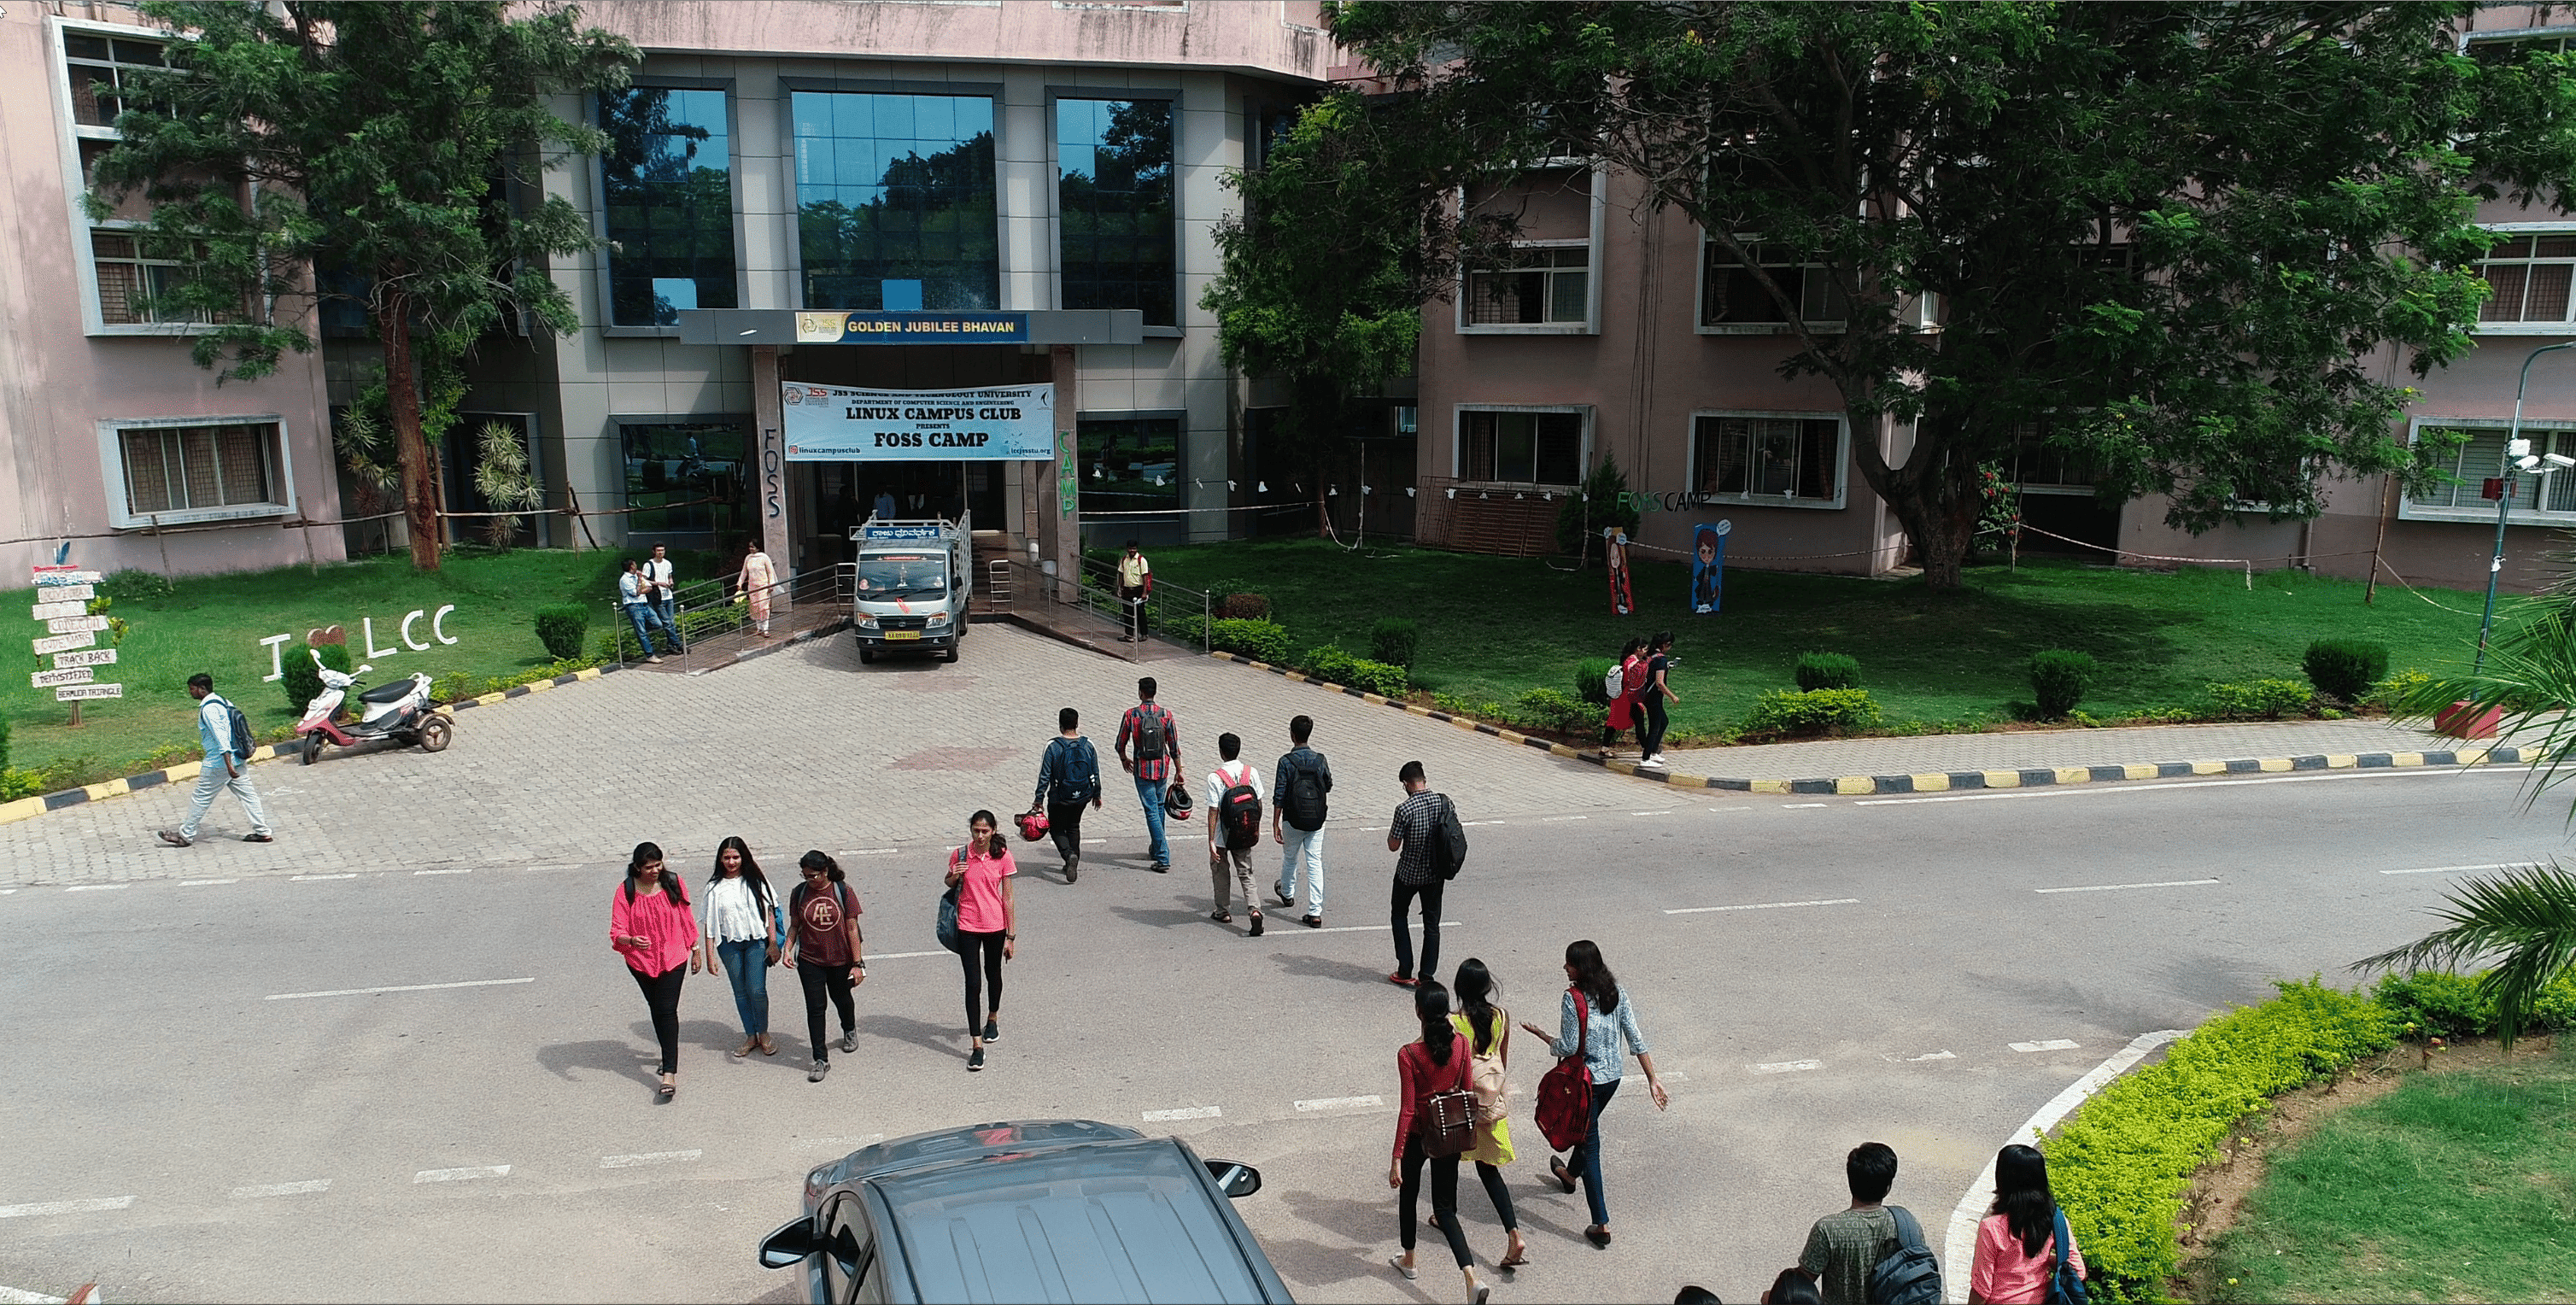
\includegraphics[width=1\textwidth]{Figure/pdestre.png}
    \caption{Sample frame from the P-DESTRE dataset showing aerial view of pedestrians captured by UAV over university campus in Portugal}
    \label{fig:pdestre_overview}
\end{figure}

Data was collected using DJI Phantom 4 drones, operated by human controllers, over university campuses in Portugal and India. The acquisition simulated everyday crowded outdoor urban environments (as shown in Figure \ref{fig:pdestre_overview}). Volunteers participated willingly, ignoring the UAVs which flew at altitudes between 5.5 and 6.7 meters with camera pitch angles from 45$^\circ$ to 90$^\circ$. Videos were recorded at 30 fps with 4K spatial resolution (3,840$\times$2,160).

The dataset is meticulously annotated at the frame level by human experts, with each video accompanied by a text file. The annotation process involved human detection, tracking, and detailed identification and soft biometrics characterization, yielding three main categories of meta-data:
\begin{enumerate}
\item \textbf{Bounding Boxes:} Precise rectangular bounding boxes for each pedestrian, supporting object detection, tracking, and semantic segmentation.
\item \textbf{Soft Biometrics Labels:} 16 distinct qualitative and quantitative labels per pedestrian (e.g., gender, age, ethnicity, hair colour, clothing information), valuable for soft biometrics and action recognition.
\item \textbf{Unique IDs:} Consistent unique identifiers for each pedestrian across multiple days and sessions, crucial for person search. Unknown identities are also annotated as distractors.
\end{enumerate}

For this dataset, we utilize the detailed cropped and annotated person bounding boxes across all videos to train the gender classification model using EfficientNet-B0.

\subsection{CUHK03}
\label{sec:cuhk03}
The CUHK03 dataset \cite{cuhk03} comprises 14,097 images of 1,467 distinct individuals. These images were captured by six campus cameras, with each person recorded by two different cameras. The dataset offers two types of bounding box annotations: one derived from manual labeling and another automatically generated by a detector. For training and testing, the dataset is divided into 20 partitions, with 100 identities specifically reserved for testing and the remainder for training. This dataset is considered highly suitable for ReID tasks due to its images being primarily captured from outdoor cameras, which introduces variability in lighting conditions and camera angles. Its relatively small number of training images poses a significant challenge for current models, often resulting in lower mean Average Precision (mAP) and Cumulative Matching Characteristics (CMC) scores compared to other datasets with similar objectives. This underscores its difficulty and importance as a benchmark for evaluating Re-ID models

\subsection{BK6I}
\label{sec:bk6i}

The BK6I dataset was captured by a group of students in the BKAI Computer Vision lab. It contains four pairs of videos representing six identities under various challenging conditions including: varying lighting conditions, different camera angles (medium and high altitude similar to UAV perspectives), occlusion scenarios, overlapping subjects, and inconsistent movement speeds. These diverse conditions make the dataset highly representative of practical surveillance environments. We utilized this dataset to evaluate the performance of the complete Re-ID pipeline.

\begin{figure}[htbp]
    \centering
    \begin{subfigure}[b]{0.48\textwidth}
        \centering
        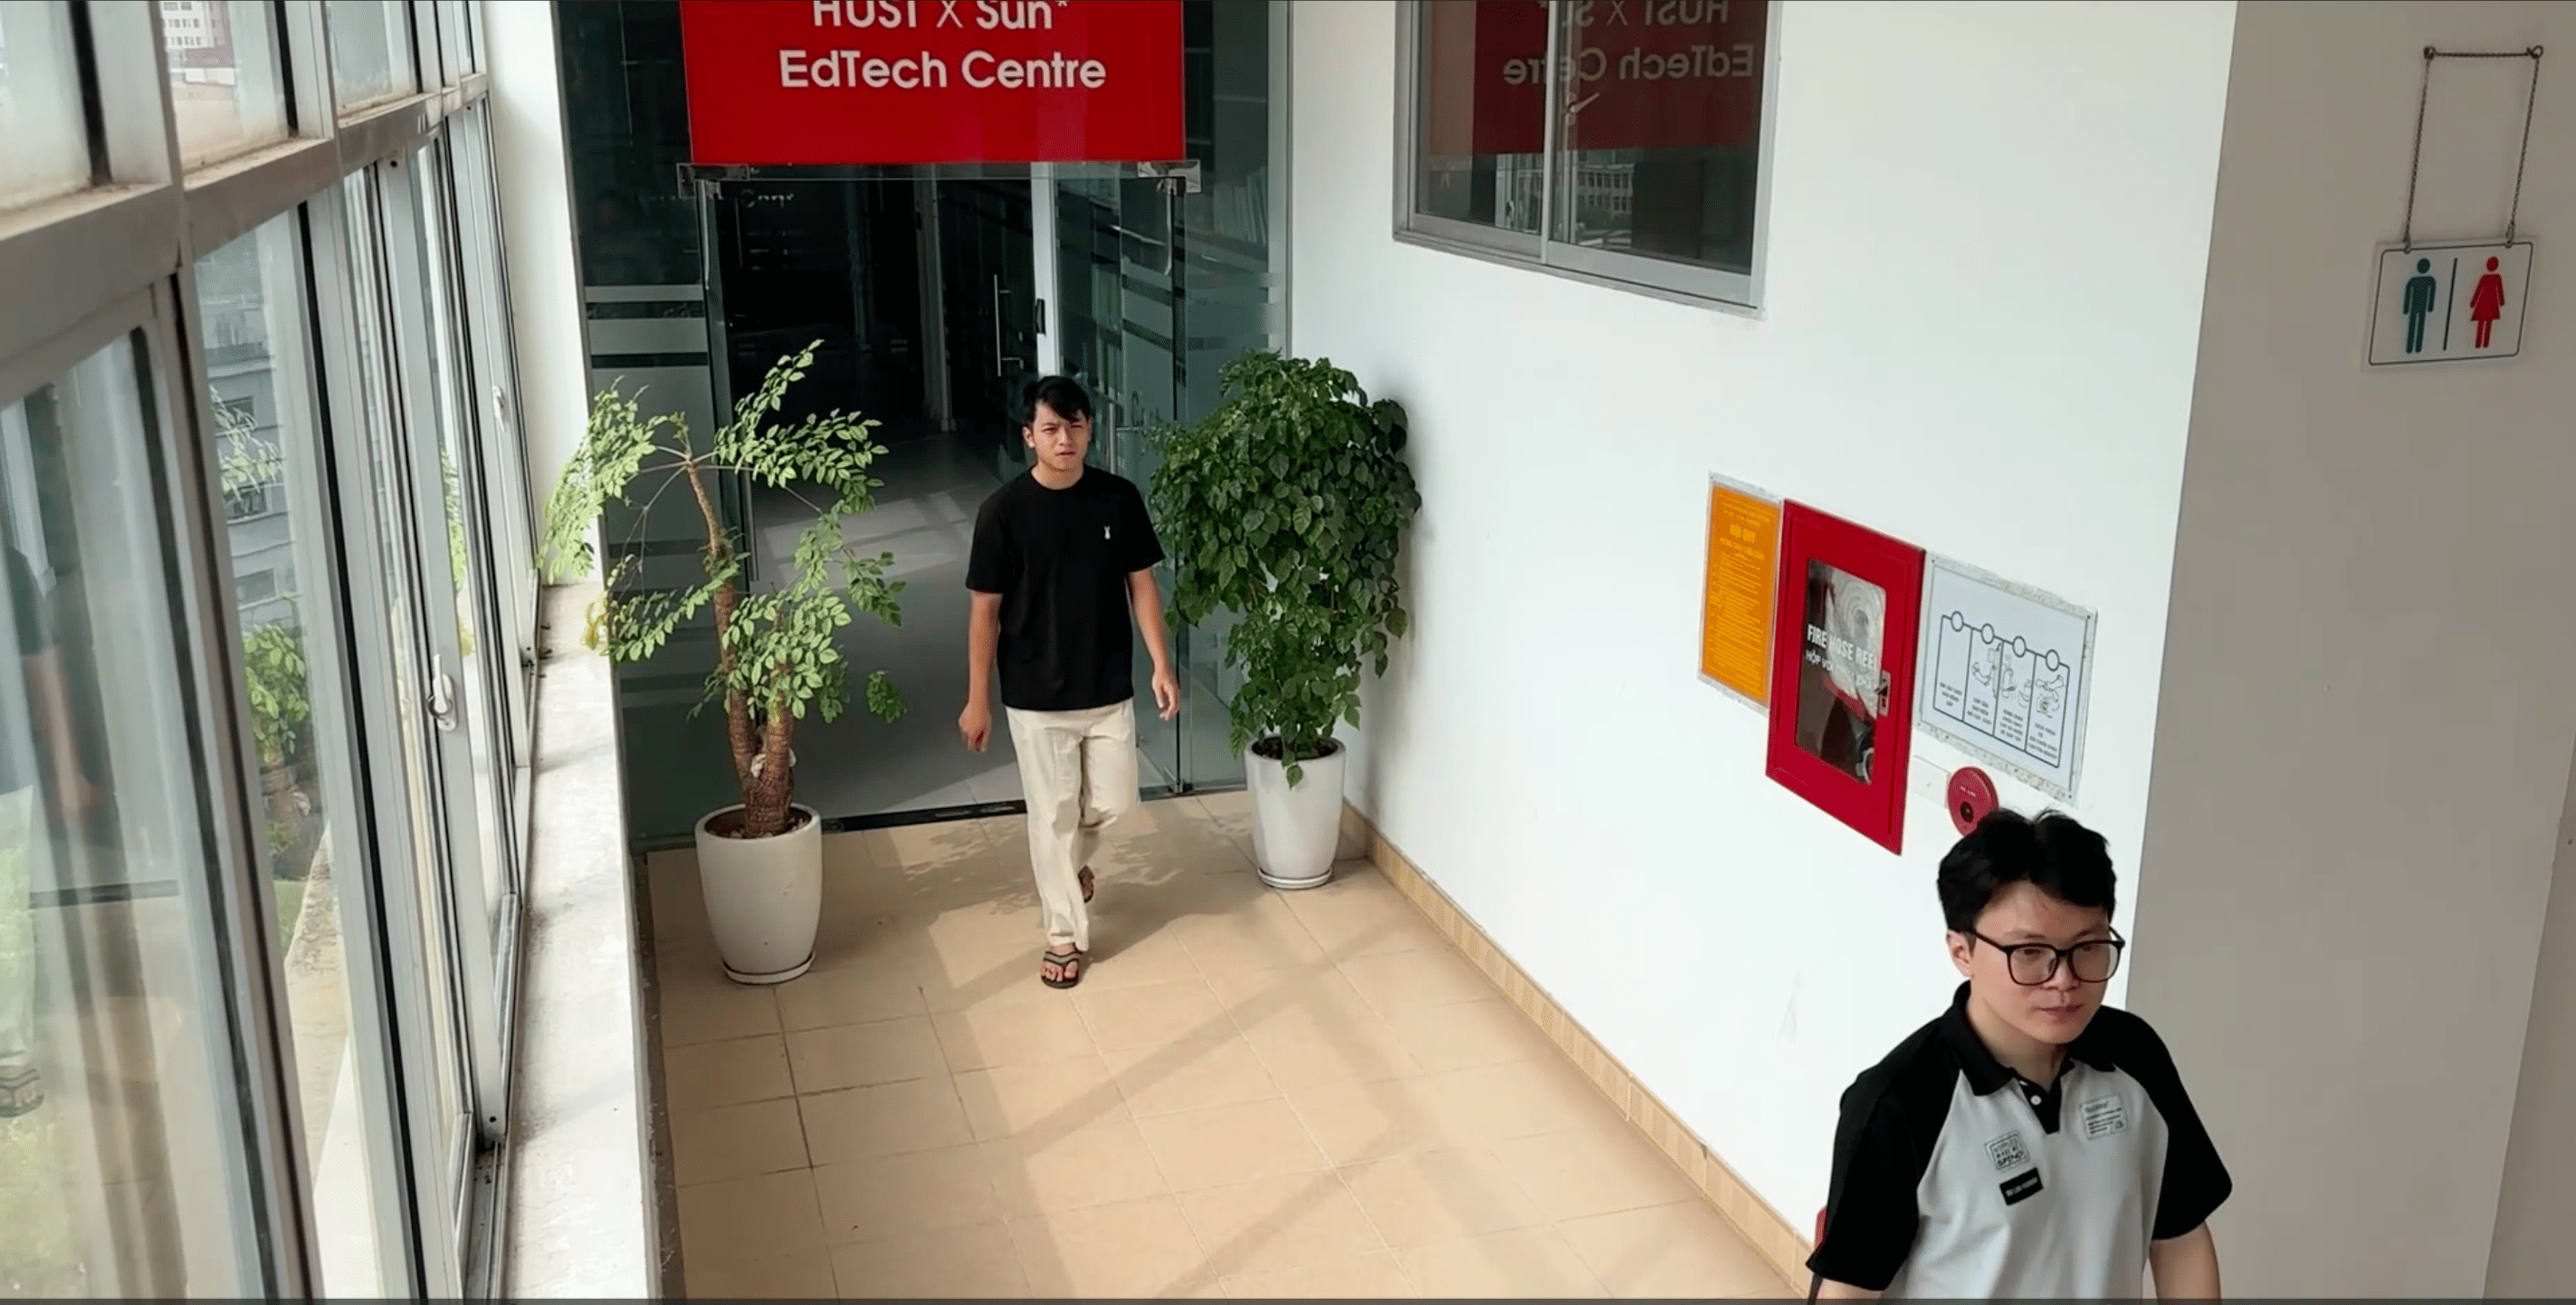
\includegraphics[width=\textwidth]{Figure/edtech_high.png}
        \caption{High altitude view}
        \label{fig:edtech_high1}
    \end{subfigure}
    \hfill
    \begin{subfigure}[b]{0.48\textwidth}
        \centering
        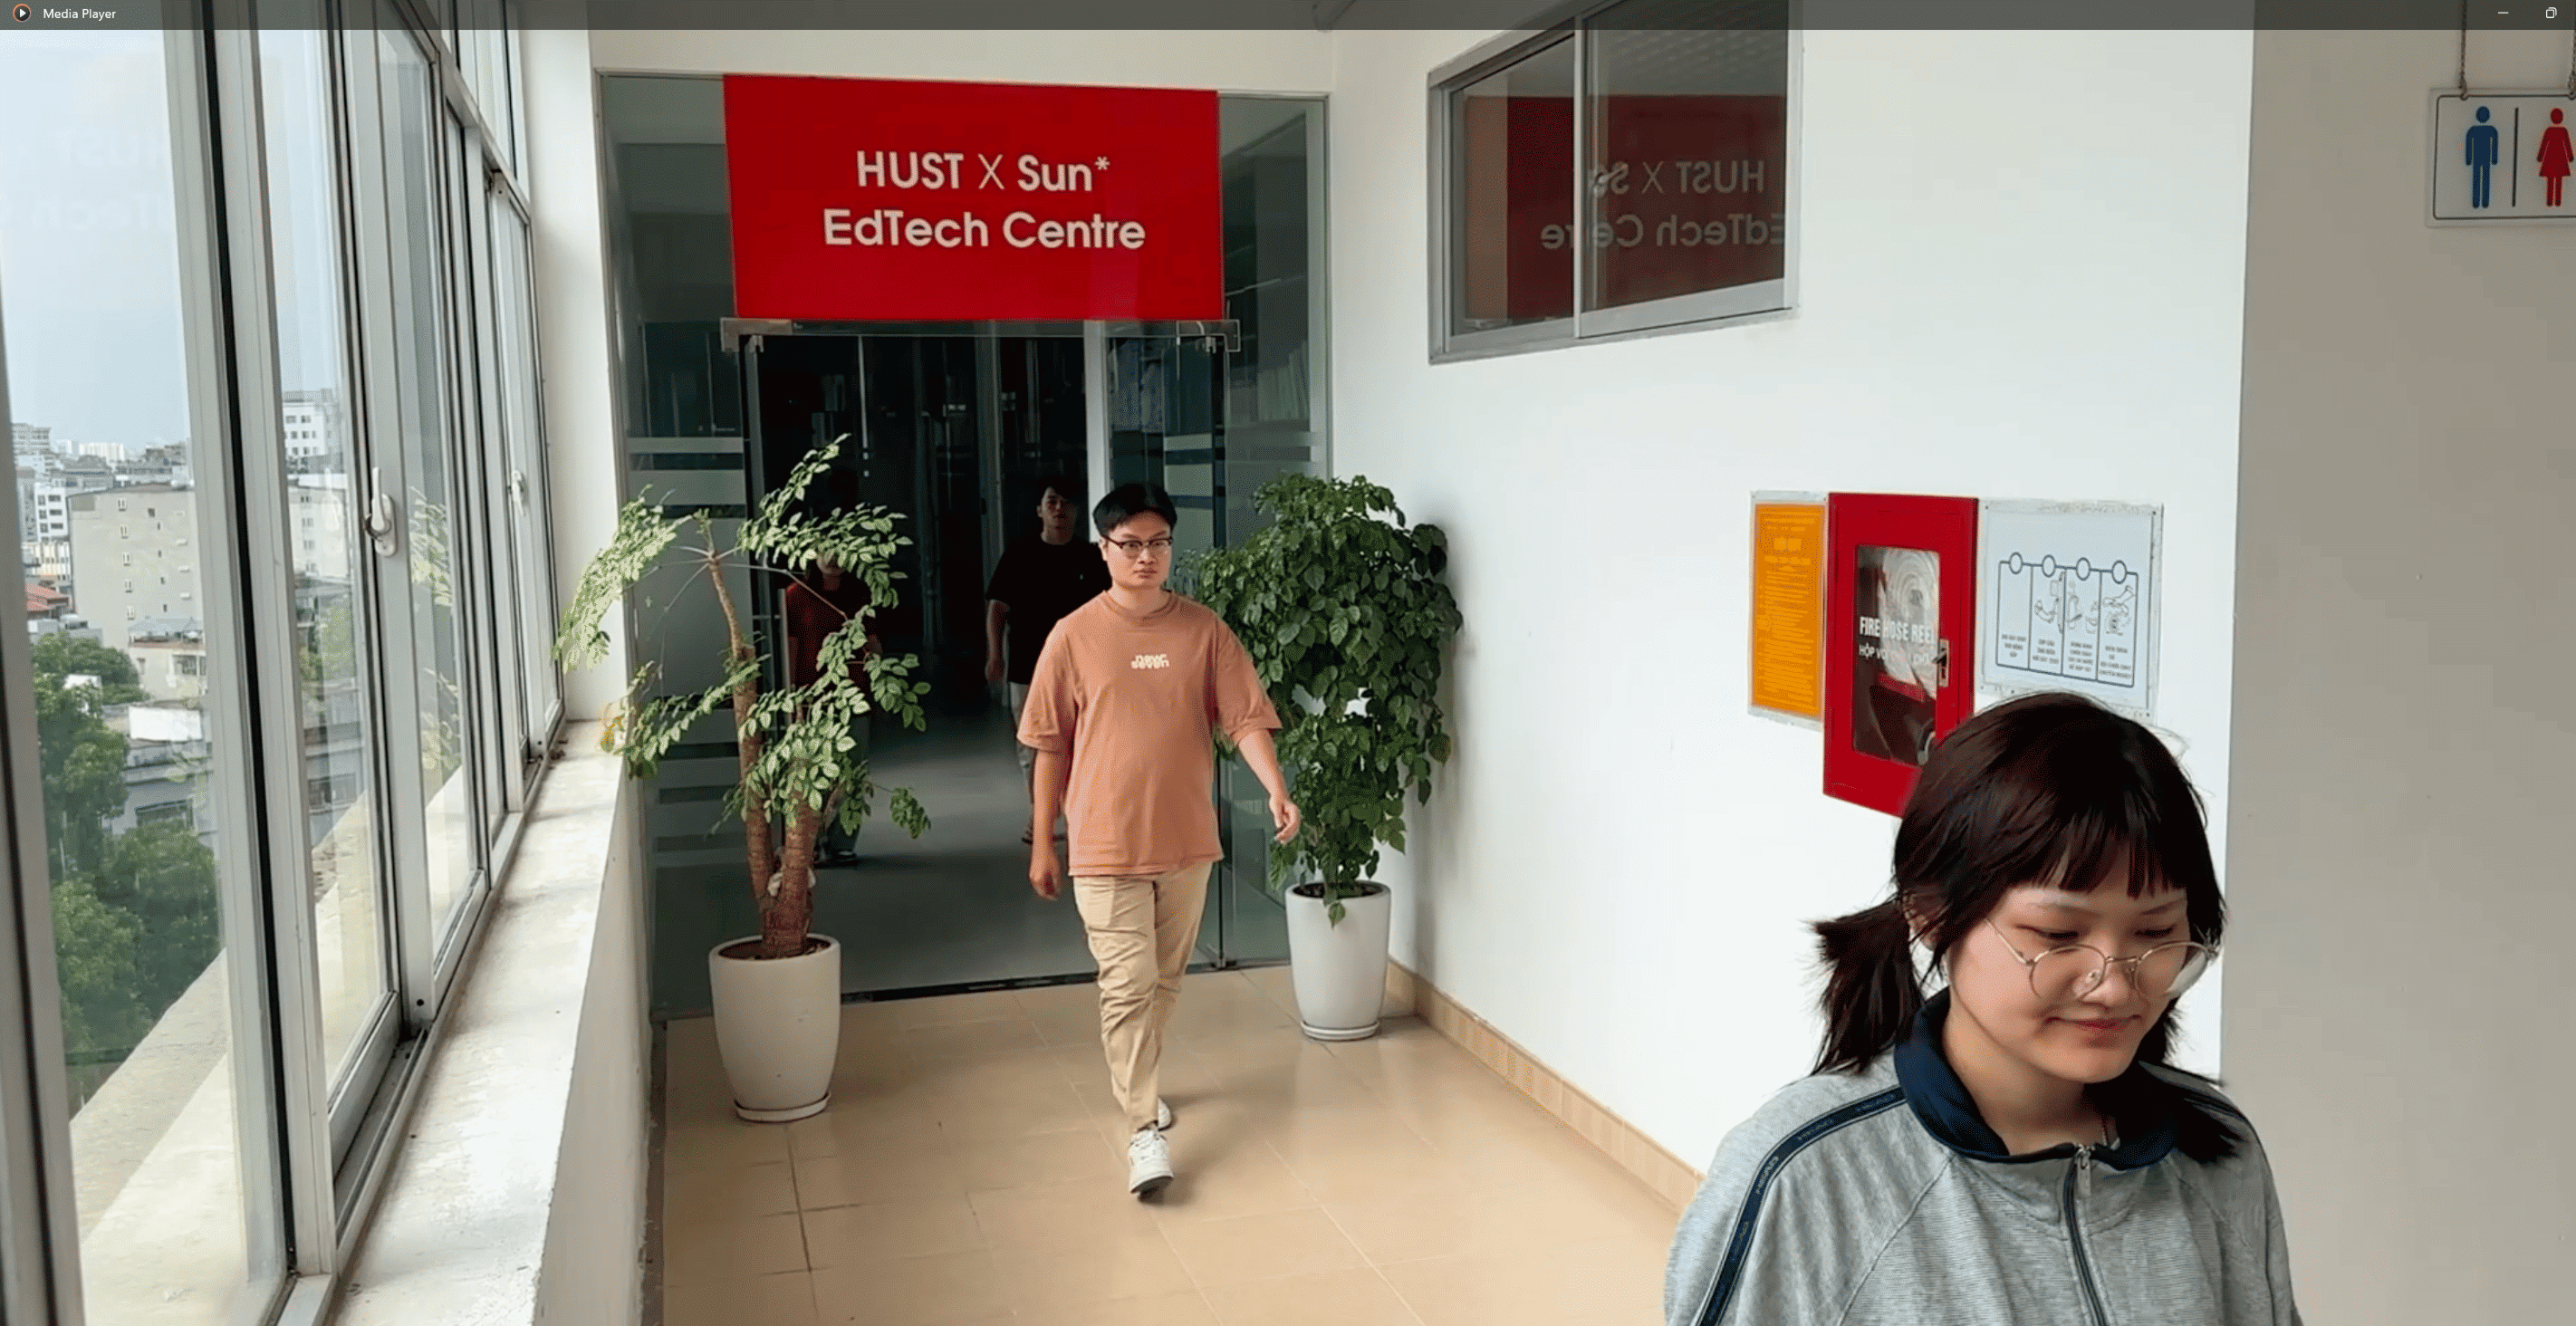
\includegraphics[width=\textwidth]{Figure/edtech_low.png}
        \caption{Low altitude view}
        \label{fig:edtech_low1}
    \end{subfigure}
    \caption{First pair of BK6I dataset samples showing different altitude perspectives}
    \label{fig:bk6i_pair1}
\end{figure}

\begin{figure}[htbp]
    \centering
    \begin{subfigure}[b]{0.48\textwidth}
        \centering
        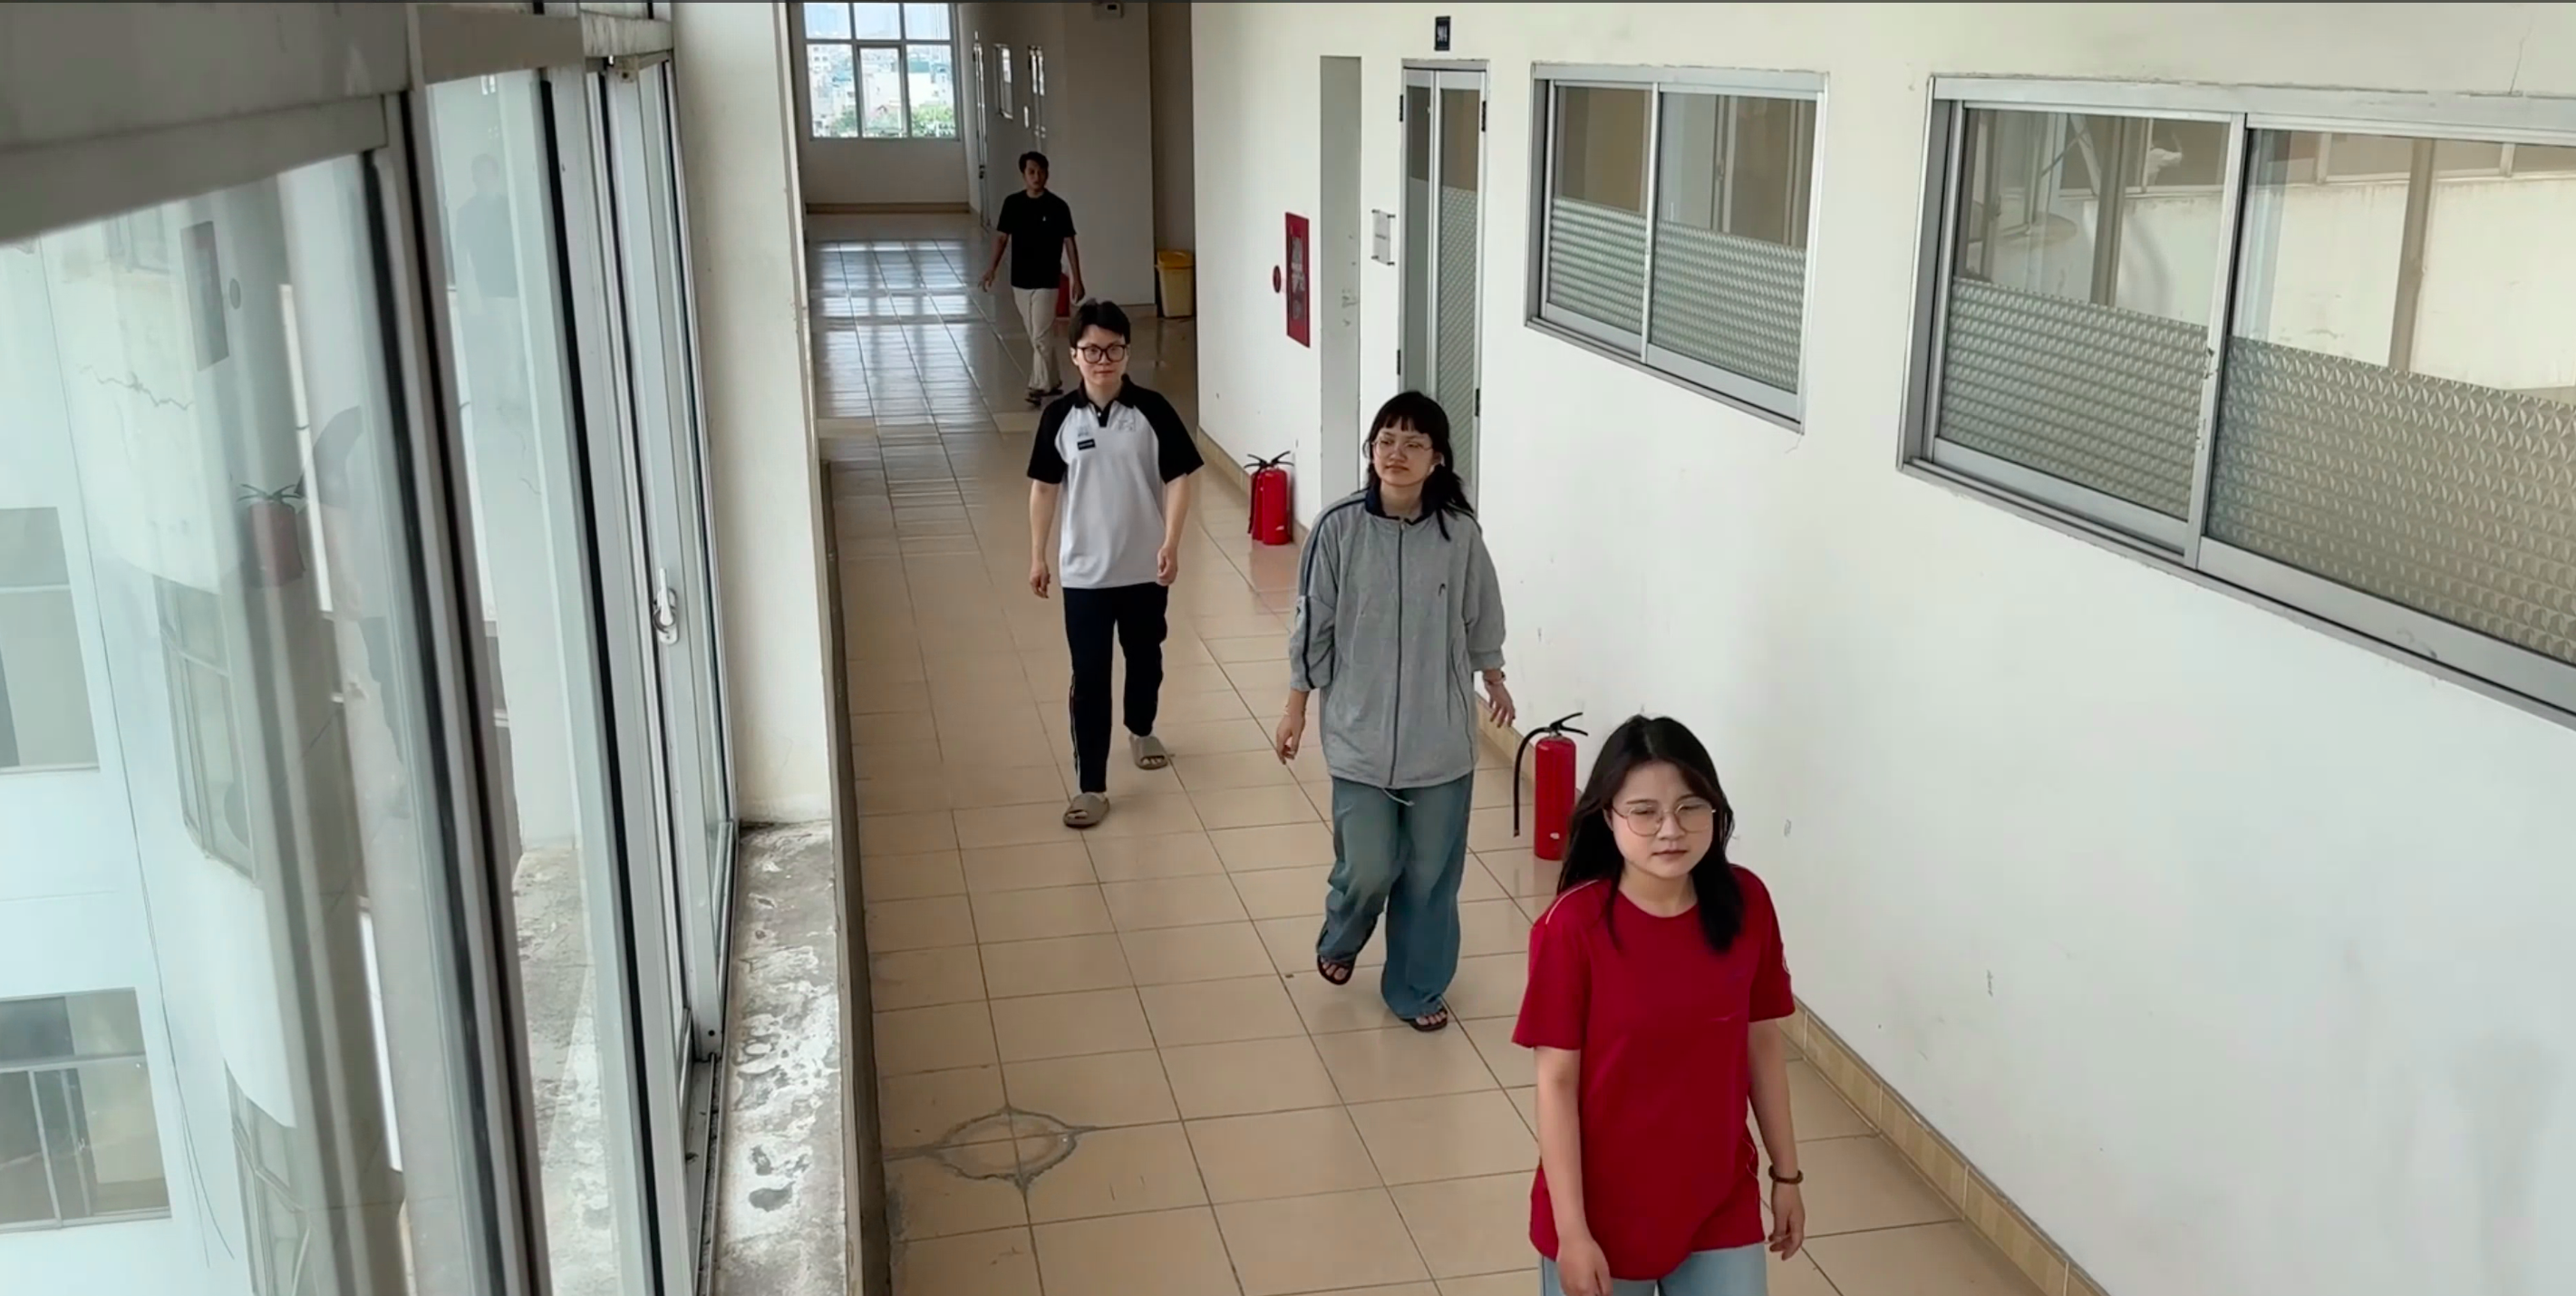
\includegraphics[width=\textwidth]{Figure/edtech_high_2.png}
        \caption{High altitude view}
        \label{fig:edtech_high2}
    \end{subfigure}
    \hfill
    \begin{subfigure}[b]{0.48\textwidth}
        \centering
        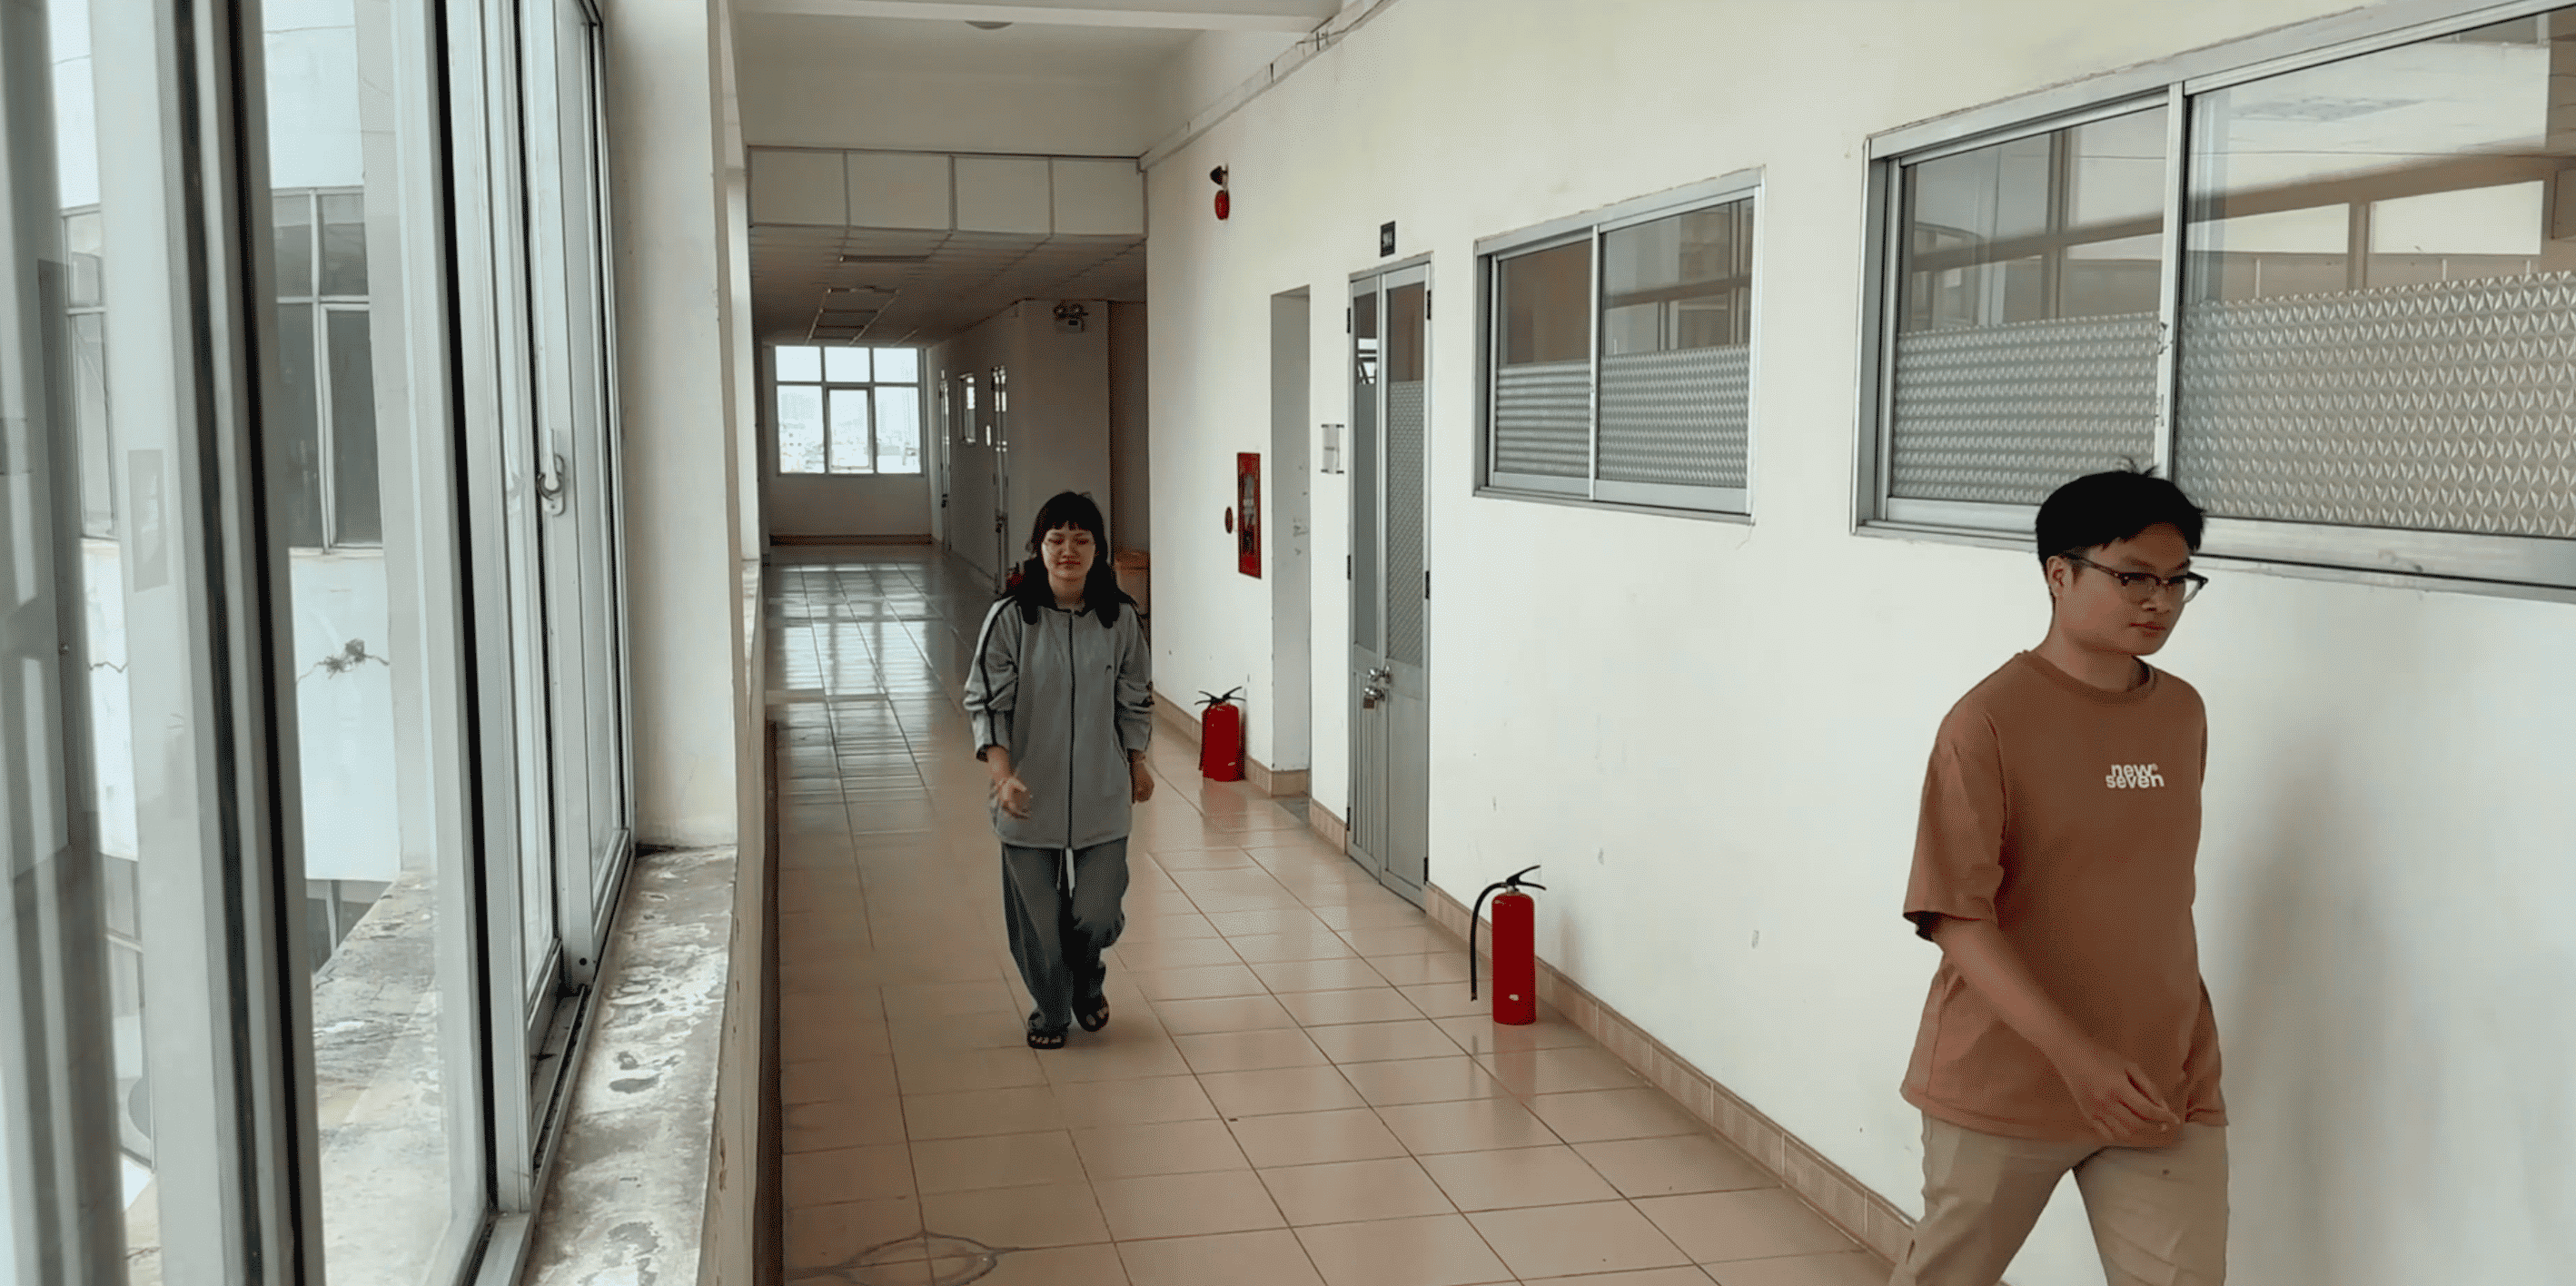
\includegraphics[width=\textwidth]{Figure/edtech_low_2.png}
        \caption{Low altitude view}
        \label{fig:edtech_low2}
    \end{subfigure}
    \caption{Second pair of BK6I dataset samples showing different altitude perspectives}
    \label{fig:bk6i_pair2}
\end{figure}

\begin{figure}[htbp]
    \centering
    \begin{subfigure}[b]{0.48\textwidth}
        \centering
        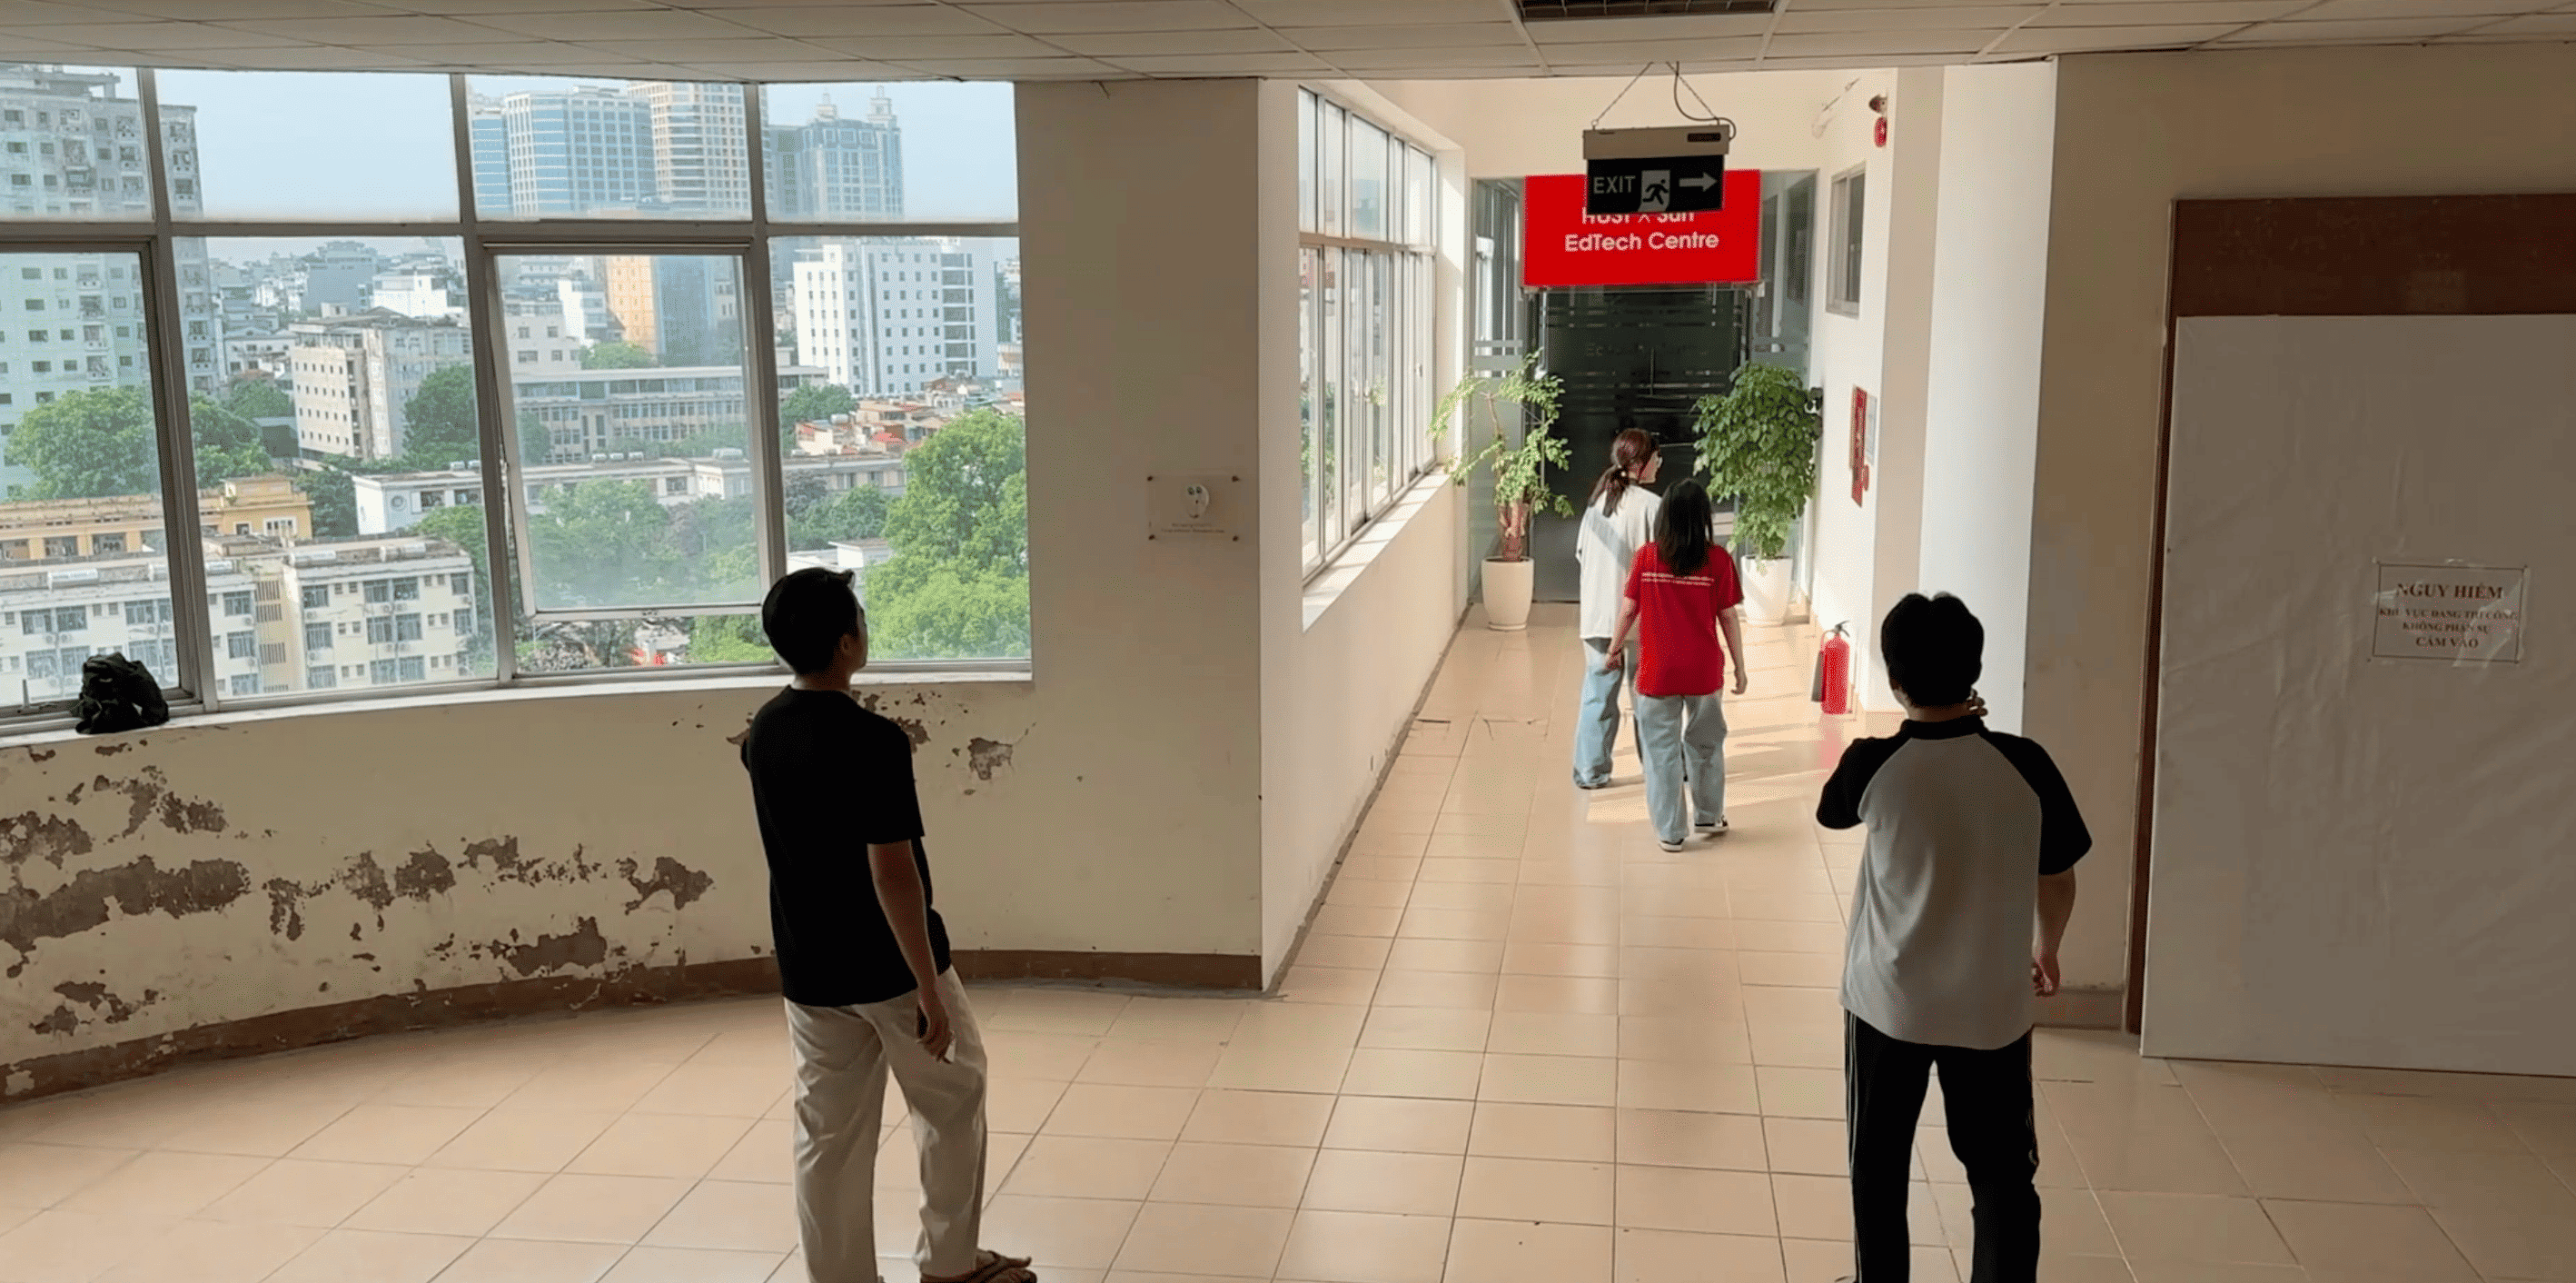
\includegraphics[width=\textwidth]{Figure/overlap_1.png}
        \caption{Overlap view from first camera}
        \label{fig:overlap1}
    \end{subfigure}
    \hfill
    \begin{subfigure}[b]{0.48\textwidth}
        \centering
        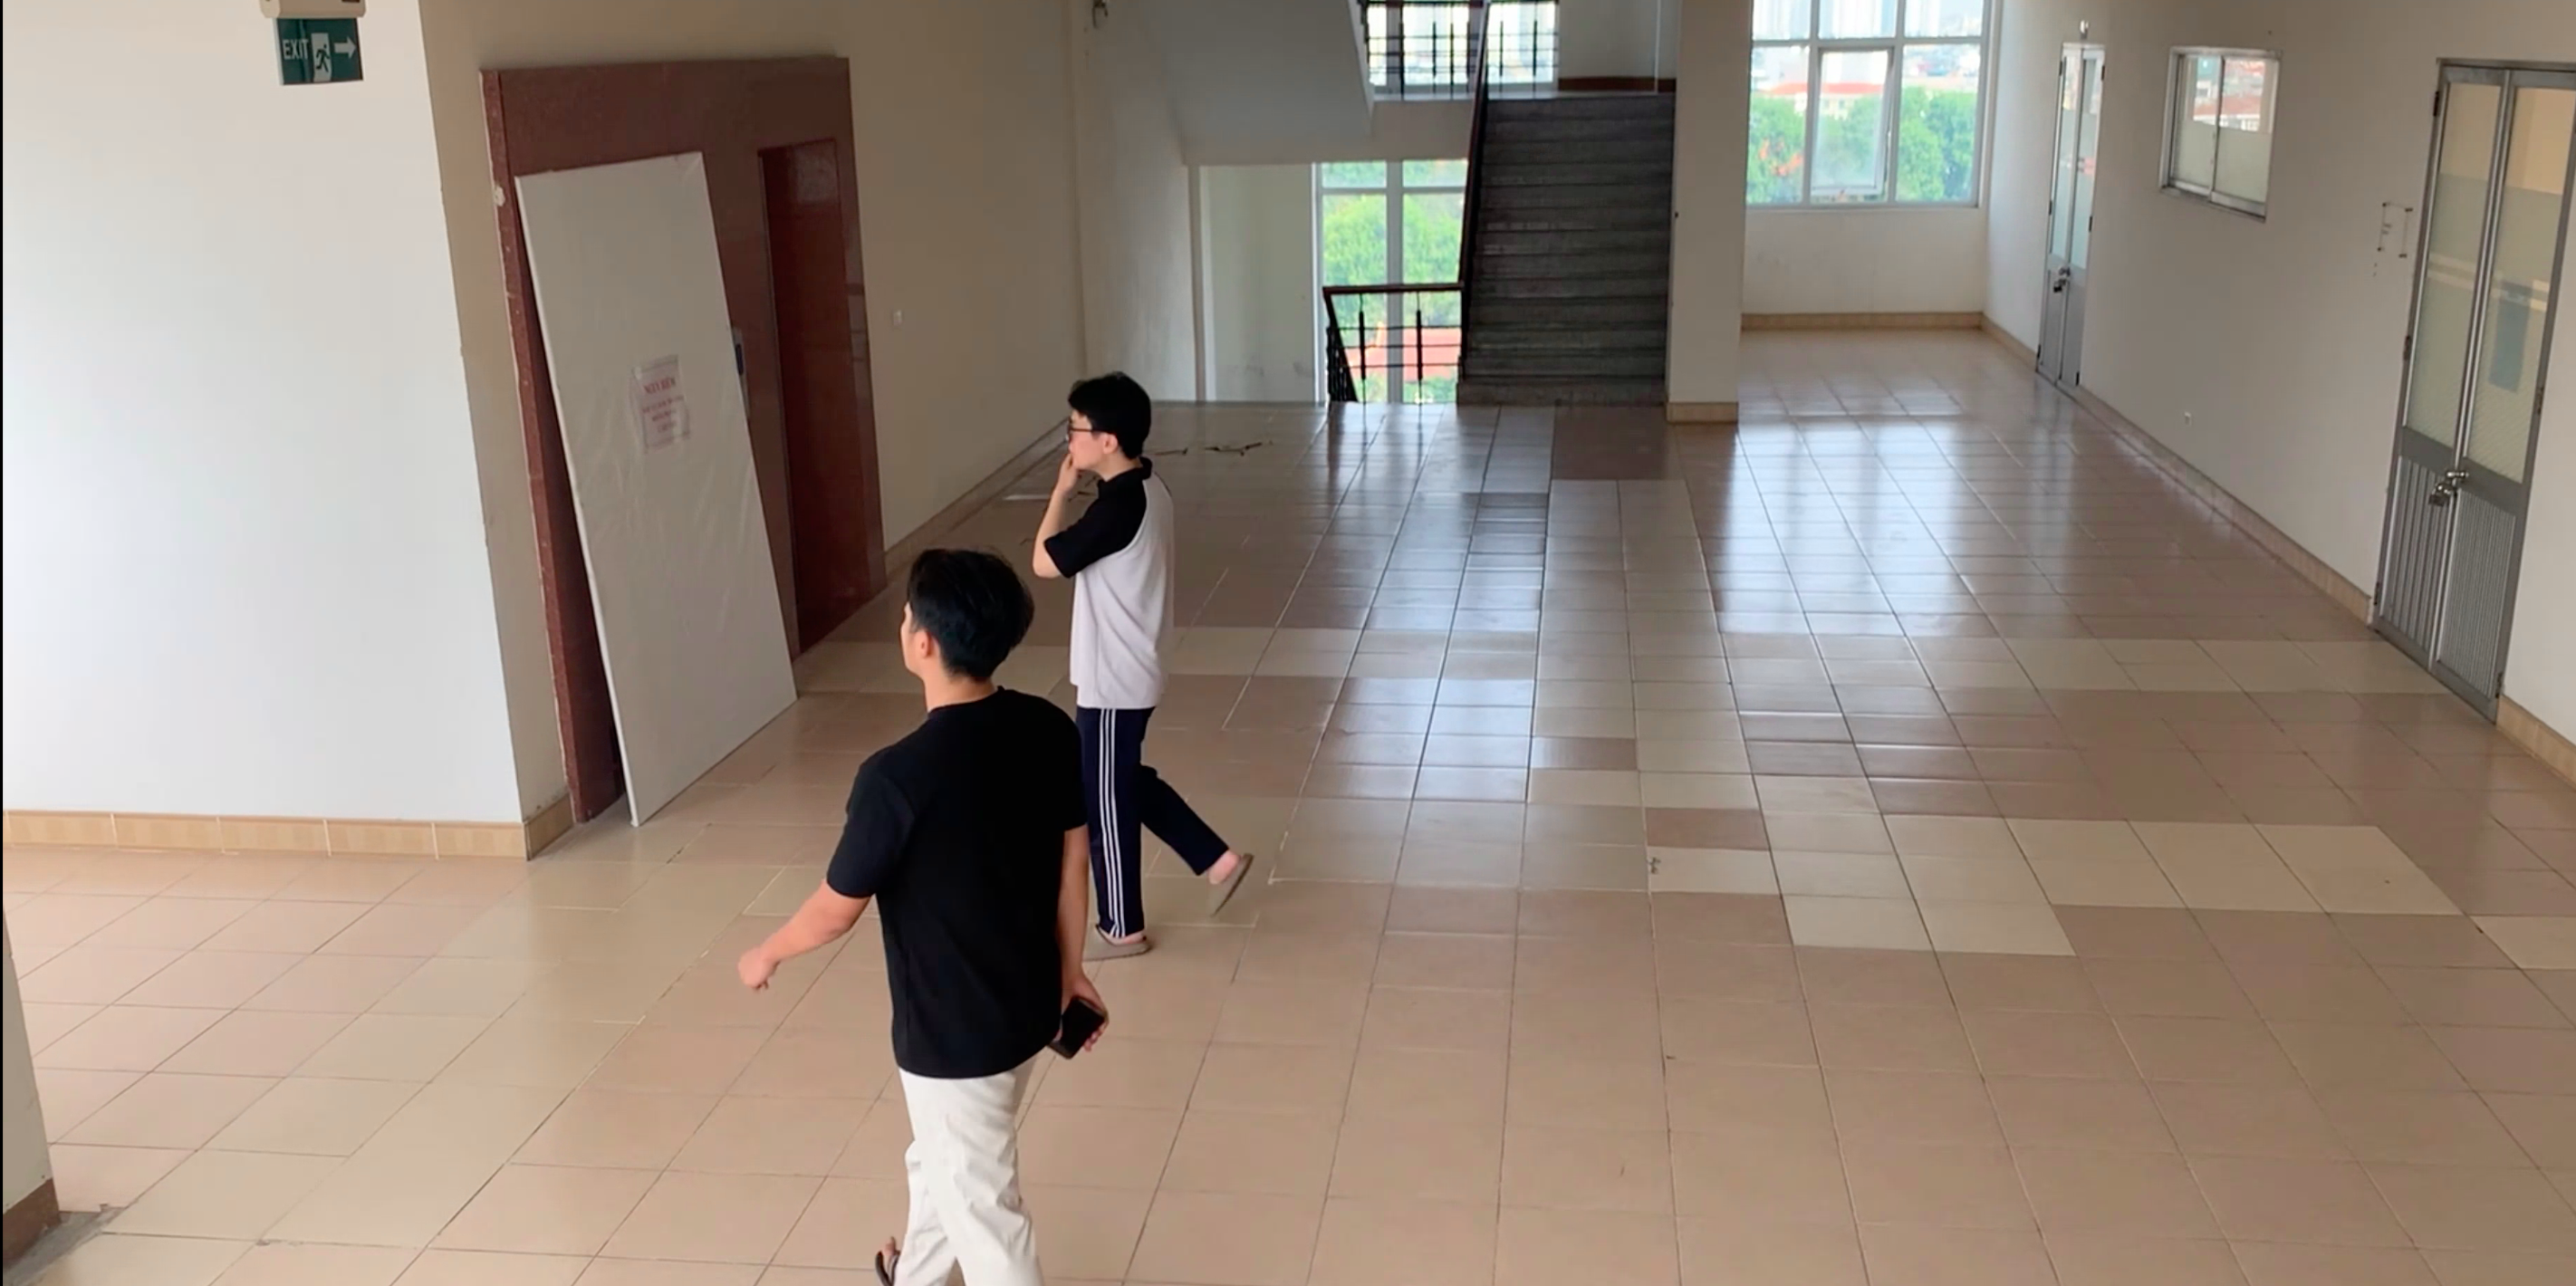
\includegraphics[width=\textwidth]{Figure/overlap_2.png}
        \caption{Overlap view 2}
        \label{fig:overlap2}
    \end{subfigure}
    \caption{Overlap view of BK6I dataset recorded from two different cameras with different angle and lighting conditions}
    \label{fig:overlap}
\end{figure}


